\documentclass[a4paper,14pt]{extreport}
%\usepackage{vntex}
\usepackage[utf8]{vietnam} %language
\usepackage{indentfirst}
\usepackage[section]{placeins}
\usepackage{a4wide,amssymb,epsfig,latexsym,array,hhline,fancyhdr}
\usepackage[table]{xcolor}
\usepackage{amsmath,mathtools,amsfonts,amsthm}
\usepackage{float}
\usepackage{color} %red, green, blue, yellow, cyan, magenta, black, white
\usepackage{diagbox}%Make diagonal lines in tables
\usepackage{caption,subcaption}
\usepackage{lmodern}
\usepackage{geometry}
 \geometry{
 a4paper,
 left=30mm,
 top=20mm,
 }

\newcommand*\plus{+{}}
\newcommand*\boxSizeOfMax[1]{\makebox[\widthof{Max}][c]{#1}}
\usepackage{lastpage}
%\usepackage{tcolorbox}
\usepackage[lined,boxed,commentsnumbered]{algorithm2e}
\usepackage{enumerate}
\usepackage{graphicx}							% Standard graphics package
\usepackage{tabularx}
\usepackage{multirow}
\usepackage{hyperref}
\usepackage[hyphenbreaks]{breakurl}
\hypersetup{
   colorlinks=true, 
   linkcolor=black,
  filecolor=magenta,      
   urlcolor=cyan,
    pdftitle={Sharelatex Example},
    bookmarks=true,
    pdfpagemode=FullScreen,
 citecolor = blue
}
 
\urlstyle{same}
\usepackage{tocbibind} %Adds "References" to the table of contents

\setlength{\headheight}{40pt}
\pagestyle{fancy}
\fancyhead{} % clear all header fields
\fancyhead[L]{
 \begin{tabular}{rl}
    \begin{picture}(25,15)(0,0)
    \put(0,-8){
\includegraphics[width=8mm, height=8mm]{img/hcmut.png}}
   \end{picture}&
	\begin{tabular}{l}
		\textbf{\bf \ttfamily Trường Đại Học Bách Khoa Tp.Hồ Chí Minh}\\
		\textbf{\bf \ttfamily Khoa Khoa Học và Kỹ Thuật Máy Tính}
	\end{tabular} 	
 \end{tabular}
}
\fancyhead[R]{
	\begin{tabular}{l}
		\tiny \bf \\
		\tiny \bf 
	\end{tabular}  }
\fancyfoot{} % clear all footer fields
\fancyfoot[L]{\scriptsize \ttfamily Đề cương luận văn tốt }
\fancyfoot[R]{\scriptsize \ttfamily Trang {\thepage}/\pageref{LastPage}}
\renewcommand{\headrulewidth}{0.3pt}
\renewcommand{\footrulewidth}{0.3pt}


%%%
\setcounter{secnumdepth}{4}
\setcounter{tocdepth}{3}
\makeatletter
%\newcounter {subsubsubsection}[subsubsection]
%\renewcommand\thesubsubsubsection{\thesubsubsection .\@alph\c@subsubsubsection}
%\newcommand\subsubsubsection{\@startsection{subsubsubsection}{4}{\z@}%
%                                     {-3.25ex\@plus -1ex \@minus -.2ex}%
%                                     {1.5ex \@plus .2ex}%
%                                     {\normalfont\normalsize\bfseries}}
%\newcommand*\l@subsubsubsection{\@dottedtocline{3}{10.0em}{4.1em}}
%\newcommand*{\subsubsubsectionmark}[1]{}
\makeatother

%\everymath{\color{blue}}%make in-line maths symbols blue to read/check easily

\sloppy
\setlength{\floatsep}{5pt plus 2pt minus 2pt}
\setlength{\textfloatsep}{5pt plus 2pt minus 2pt}
\setlength{\intextsep}{10pt plus 2pt minus 2pt}
\begin{document}

\begin{titlepage}
    \begin{center}
    ĐẠI HỌC QUỐC GIA THÀNH PHỐ HỒ CHÍ MINH \\
    TRƯỜNG ĐẠI HỌC BÁCH KHOA \\
    KHOA KHOA HỌC - KỸ THUẬT MÁY TÍNH 
    \end{center}

    \vspace{1cm}
    
    \begin{figure}[h!]
        \begin{center}
        
\includegraphics[width=3cm]{img/hcmut.png}
        \end{center}
    \end{figure}
        
    \vspace{1cm}

    \begin{center}
        \begin{tabular}{c}
        \multicolumn{1}{l}{\textbf{{\Large Đề cương luận văn tốt nghiệp (CO4311)}}}\\
        ~~\\
        \\
        \hline
         \\
        \textbf{{\LARGE Đề tài:}} \\
		\textbf{{\LARGE Tìm kiếm đối tượng trong tập dữ liệu}}\\
		\textbf{{\LARGE ảnh dựa trên đặc trưng của đối tượng}}
		\\
		\\
        \hline
        \end{tabular}
    \end{center}

    \vspace{1.2cm}

    \begin{minipage}[t]{0.4\textwidth}
        \begin{flushleft}\large
            \emph{Giáo viên hướng dẫn:}
            \\PGS.TS. Nguyễn Thanh Bình
        \end{flushleft}
    \end{minipage}
    \begin{minipage}[t]{0.7\textwidth}
        \begin{flushright}\large
        \emph{Sinh viên thưc hiện:}\\ 
            \begin{tabular}{ c c }
                Dương Thanh Nam & 1512058\\ 
                Nguyễn Ngọc Tâm & 1620058\\  
                Nguyễn Mậu Vĩnh & 1627058\\    
            \end{tabular}
        \end{flushright}
    \end{minipage}\\

    \begin{center}
        {\footnotesize Tp. Hồ Chí Minh, Tháng 12/2018}
    \end{center}
\end{titlepage}
%New page 
\newpage
\tableofcontents

\newpage


%%%%%%%%%%%Chapter 1 Giới thiệu đề tài %%%%%%%%%%%%%%%%%%%%%
\chapter{Giới thiệu}
\section{Giới thiệu đề tài}
Với sự phát triển của Internet, cùng với những tiến bộ trong công nghệ lưu trữ dữ liệu và thu thập hình ảnh, 
nhất là xung quanh chúng ta luôn có sẵn các thiết bị để thu bắt lại các bức ảnh như máy ảnh kĩ thuật số, máy scan hình, 
điện thoại di động, tablet,... khiến cho kích thước tập dữ liệu ảnh kĩ thuật số đang tăng lên nhanh chóng. 
Với một tập hình ảnh đang ngày một lớn lên nhanh chóng như thế thì câu hỏi đặt ra là làm thế nào để tìm kiếm đối 
tượng trong tập dữ liệu hình ảnh theo nhu cầu sử dụng một cách nhanh chóng và chính xác. Câu hỏi này cũng chính là 
một nội dung được các nhà khoa học máy tính quan tâm nghiên cứu trong vài thập kỷ qua.
\par 
Các phương pháp tìm kiếm hình ảnh hiện nay có hai hướng tiếp cận chính, thứ nhất đó là tìm kiếm theo metadata của dữ liệu ảnh, thứ hai là tìm kiếm 
theo các đặc trưng được thể hiện trong chính bức ảnh đó. Tuy nhiên, với số lượng hình ảnh quá lớn, việc tiếp cận 
theo hướng tìm kiếm theo metadata tỏ ra không hiệu quả, bởi vì việc tạo metadata thủ công tốn rất nhiều thời gian 
và công sức, hơn nữa, chúng ta rất khó kiểm soát việc gắn metadata như vậy có chính xác hay không, vì nó phụ thuộc 
nhiều vào con người, ngôn ngữ và bối cảnh của hình ảnh. Để khắc phục những hạn chế này, tiếp cận bằng cách tìm kiếm 
đối tượng theo đặc trưng của ảnh được các nhà nghiên cứu quan tâm, phát triển và cũng đã đạt được nhiều kết quả đáng kể. 
\par
Các phương pháp được thực hiện theo hướng này giúp cho việc lưu trữ đặc trưng cũng như tìm kiếm đối tượng diễn ra một cách 
có hệ thống, hạn chế sự tham gia của con người trong việc tạo dữ liệu đặc trưng, qua đó tăng độ chính xác cũng như tốc 
độ khởi tạo dữ liệu trong cơ sở dữ liệu hình ảnh.
\par
Trong đề cương luận văn này, nhóm sẽ tìm hiểu một số phương pháp tìm 
kiếm đối tượng theo đặc trưng đã được nghiên cứu và phát triền, đồng thời đề xuất hướng hiện thực một phương pháp trong 
đó cho luận văn sắp tới.


\section{Mục tiêu, nội dung đề tài}

\subsection{Mục tiêu}
Mục tiêu của đề tài là hiện thực một phương pháp tìm kiếm đối tượng theo đặc trưng của hình ảnh trong tập dữ liệu lớn.

\subsection{Nội dung đề tài}
Nội dung chính của đề tài bao gồm các những phần sau đây:
\begin{enumerate}
    \item Tìm hiểu các định dạng ảnh số.
    \item Tìm hiểu các công trình nghiên cứu liên quan đến đề tài.
    \item Đề xuất phương pháp tìm kiếm đối tượng dựa trên đặc trưng.
    \item Hiện thực, so sánh kết quả với các giải thuật khác.
    \item Đánh giá kết quả đạt được.
\end{enumerate}

% \section{Giới hạn đề tài}
%  Trong bài luận văn này, nhóm sẽ chỉ nghiên cứu về phương pháp tìm kiếm cho các ảnh chỉ chứa một đối tượng, và đối tượng này sẽ chiếm phần lớn nội dung của bức ảnh, 
% đồng thời bức ảnh cũng thể hiện đầy đủ đối tượng. Ví dụ bức ảnh sẽ chỉ chứa một chiếc xe hơi được chụp ở khoảng cách gần, bức ảnh sẽ thể hiện đầy đủ chiếc xe hơi, 
% đồng thời nội dung bức ảnh sẽ chủ yếu thể hiện chiếc xe hơi, không phải một đoạn đường có nhiều xe hơn hoặc một chiếc xe hơi rất nhỏ nằm trong một khung cảnh lớn.

% \section{Cấu trúc luận văn}
% Nội dung bài luận văn này được chia thành 5 chương như sau:
% \par
% \textbf{Chương 1:} Giới thiệu về nội dung đề tài, tính cần thiết của đề tài và phạm vi nghiên cứu của nhóm.
% \par
% \textbf{Chương 2:} Trình bày cơ sở lí thuyết về hình ảnh, các phương pháp trích xuất đặc trưng ảnh và các phương pháp đo lường độ tương đồng của hình ảnh dựa trên đặc trưng trích xuất được. Ngoài ra chương này còn trình bày tóm lược về các nguyên cứu liên quan và những kết quả  mà các nghiên cứu này đã đạt được.
% \par
% \textbf{Chương 3:} Yêu cầu của bài toán, các giải thuật mà nhóm đề xuất nghiên cứu và phương pháp để đánh giá kết quả đạt được.
% \par
% \textbf{Chương 4:} Hiện thực chương trình đơn giản một tập dữ liệu nhỏ để minh họa cho các nghiên cứu của nhóm. 
% \par
% \textbf{Chương 5:} Chương này sẽ nêu ra các kết quả đạt được, ưu nhược điểm và định hướng cho luận văn tốt nghiệp của nhóm.

% % %%%%%%%%%%%%%%%Chapter 2 Cở sở lí thuyết và các nghiên cuuw liên quan%%%%%%%%%%%%%%%%%%%%
% \chapter{Cơ sở lí thuyết và các nghiên cứu liên quan}
% \section{Cơ sở lí thuyết}
% \subsection{Ảnh số}
% \textbf{Ảnh số} là đại diện của hình ảnh thực, là một tập hợp những con số được lưu trữ, xử lý bởi máy tính số. Để chuyển hình ảnh thành số, hình ảnh được chia thành các khu vực nhỏ gọi là pixel. Đối với mỗi pixel, thiết bị hình ảnh ghi lại một số hoặc một bộ số nhỏ mô tả một số thuộc tính của pixel này, chẳng hạn như độ sáng của nó hoặc màu của nó. Các số được sắp xếp trong một mảng các hàng và cột tương ứng với vị trí dọc và ngang của các pixel trong ảnh.\cite{img-defi} Mỗi số có giá trị trong khoảng 0 - 255. Với ảnh màu ta sẽ có ba ma trận hai chiều. Mỗi ma trận là một kênh màu của ảnh. Ba ma trận tương ứng với ba kênh màu Red, Green và Blue đối với ảnh RGB. Giá trị tại một pixel trên ảnh là tổng hợp ba giá trị tại vị trí tương ứng ở ba ma trận trên.  
% \\
% Hình ảnh kỹ thuật số có một số đặc điểm cơ bản:

% \begin{itemize}
%     \item Loại hình ảnh. Ví dụ, hình ảnh đen trắng chỉ ghi lại cường độ ánh sáng trên các pixel. Một hình ảnh màu có thể có ba màu, thường là RGB (Đỏ, Xanh lục, Xanh lam) hoặc bốn màu, CMYK (Cyan, Magenta, Yellow, blacK). (ppi).\cite{img-defi}
%     \item Độ phân giải. Độ phân giải được thể hiện bằng số pixel trên mỗi inch (ppi). Độ phân giải cao hơn cho hình ảnh chi tiết hơn. Một màn hình máy tính thường có độ phân giải 100 ppi, trong khi máy in có độ phân giải từ 300 ppi đến hơn 1440 ppi. Đây là lý do tại sao một hình ảnh được in trông tốt hơn nhiều so với trên màn hình.\cite{img-defi}
%     \item Độ sâu màu (của hình ảnh màu) hoặc "bit trên pixel" là số lượng bit mô tả độ sáng hoặc màu. Nhiều bit hơn có thể ghi lại nhiều sắc thái của màu xám hoặc nhiều màu hơn.\cite{img-defi}
%     \item Định dạng của hình ảnh cung cấp thêm chi tiết về cách các số được sắp xếp trong tệp hình ảnh, bao gồm loại nén nào được sử dụng (nếu có). Các định dạng phổ biến nhất là JPG, PNG, GIF, TIFF, và BMP.\cite{img-defi}
% \end{itemize}
% \subsection{Các định dạng ảnh số}
% \subsubsection*{a) Định dạng ảnh JPG}

% File JPG hay còn gọi là các tập tin JPEG, là một định dạng ảnh kỹ thuật số phổ biến. Định dạng JPG được lưu với thuật toán nén lossy, điều này đồng nghĩa với việc chất lượng hình ảnh sẽ bị giảm đi và kích thước tập tin cũng được giảm đáng kể.\cite{img-format}

% Ưu điểm của JPG/JPEG:

% \begin{itemize}
%     \item Độ sâu màu từ 24 bit đến 16 triệu màu.
%     \item JPEG là chuẩn hình ảnh thông dụng nhất cho hầu hết các máy ảnh số hiện nay.
%     \item JPEG tương thích với mọi trình duyệt web hiện nay.
%     \item Sử dụng tốt nhất, hiệu quả nhất cho ảnh trắng đen, ảnh với màu sắc phức tạp, ảnh tĩnh vật, ảnh đời thường, chân dung.
% \end{itemize}

% \subsubsection*{b) Định dạng ảnh PNG}

% PNG (Portable Network Graphics) là một định dạng tập tin đồ họa raster, hỗ trợ nén dữ liệu không bị suy giảm chất lượng, được sử dụng rất nhiều trên internet.\cite{img-format}

% Ưu điểm của PNG:

% \begin{itemize}
%     \item Nén theo chuẩn LossLess, có nghĩa là hình ảnh sau khi bị nén vẫn giữ nguyên được chất lượng.
%     \item Định dạng PNG sử dụng tốt trên web/blog, những mảng màu phẳng, thiết kế Logo, hình ảnh có nền trong suốt hoặc bán trong suốt.
%     \item Thích hợp với hình ảnh đơn giản như văn bản.
% \end{itemize}

% \subsubsection*{c) Định dạng ảnh GIF}

% GIF thường được dùng cho hình ảnh trên web, GIF sử dụng thuật nén Lossless mà không làm giảm chất lượng hình ảnh sau khi nén. GIF lưu dữ liệu bằng cách sử dụng màu indexed, có nghĩa là mỗi hình ảnh có thể bao gồm 256 màu.\cite{img-format}

% Ưu điểm của GIF:

% \begin{itemize}
%     \item GIF hỗ trợ ít màu nên các tập tin thường có dung lượng nhỏ hơn JPGE rất nhiều.
%     \item Hình ảnh được nén theo chuẩn Lossless nên không bị mất dữ liệu khi nén.
%     \item GIF sống động với hình ảnh động.
% \end{itemize}

% \subsubsection*{d) Định dạng ảnh TIFF}

% TIFF (Tagged Image Format File)  là một định dạng file ảnh chất lượng cao và được sử dụng nhiều cho việc Scan.\cite{img-format}

% Ưu điểm của TIFF:

% \begin{itemize}
%     \item Cho dù bị nén hay không nén thì file TIFF cũng không bị mất bất kỳ dữ liệu.
%     \item Do chất lượng hình ảnh của định dạng này rất tốt nên thường được sử dụng để lưu những hình ảnh có màu sắc phức tạp và thường được sử dụng để Scan.
%     \item File TIFF có thể xem được, chỉnh sửa được.
% \end{itemize}

% \subsubsection*{e) Định dạng ảnh BMP}

% Định dạng BMP là một dạng file ảnh đồ họa dạng lưới (raster) được sử dụng để lưu trữ hình ảnh kỹ thuật số bitmap.\cite{img-format} 

% Đặc điểm của BMP:

% \begin{itemize}
%     \item File BMP không hỗ trợ tốt cho việc nén hình ảnh.
%     \item Dễ dạng được tạo ra từ những dữ liệu pixel được lưu trong bộ nhớ máy tính.
%     \item File Bitmap dễ dàng được dịch ra thành định dạng điểm cho các thiết bị như màn hình CRT và máy in.
% \end{itemize}

% \subsection{ Trích xuất dữ hình ảnh theo đặc trưng } 
% Content-Based Image Retrieval (CBIR) là một ứng dụng của thị giác máy tính nhằm trích xuất các hình ảnh tương tự với hình ảnh mẫu làm đầu vào cho hệ thống. Các kĩ thuật CBIR sử dụng nội dung hiển thị của hình ảnh được mô tả dưới dạng các đặc trưng để biểu diễn và tìm kiếm hình ảnh trong tập dữ liệu. CBIR là kĩ thuật đáng tin cậy vì hầu hết các công cụ tìm kiếm hình ảnh dựa trên web dựa hoàn toàn vào metadata và điều này rất tốn thời gian, tạo ra rất nhiều kết quả rác. 

% Người dùng có thể query hệ thống CBIR theo nhiều cách khác nhau, có thể là query theo một hình ảnh đầu vào, theo caption, theo một đoạn văn mô tả, theo một thuộc tình nào đó của hình ảnh. Sau đó hệ thống sẽ tìm kiếm và output những hình ảnh tương tự.

% Những hình ảnh được coi là tương tự nhau nếu chúng tương tự nhau ở các đặc điểm ở trong hình ảnh (tương tự về màu, texture..), hoặc những hình ảnh gần như giống nhau hoàn toàn, chỉ khác nhau về màu, về phóng to thu nhỏ, xoay.., hoặc chứa những vật thể giống nhau, background giống nhau...Có hai mức độ tương tự nhau là tương tự nội dung trực quan và tương tự nội dung nghữ nghĩa.

% Hình 2.1 minh họa một kiến trúc cơ bản của một hệ thống trích xuất ảnh theo đặc trưng với query là một hình ảnh đầu vào và tìm những hình ảnh tương tự dựa trên nội dung trực quan trong tập dữ liệu ảnh.

% \begin{figure}[h] 
%     \centering
%     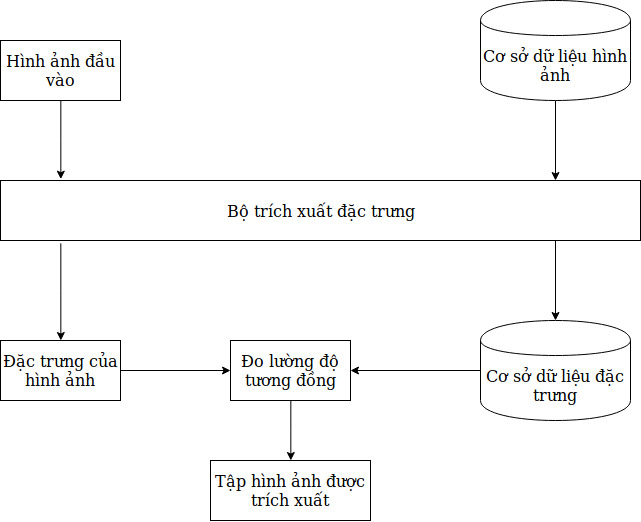
\includegraphics[scale=0.5]{img/cbri-architect.jpg}
%     \caption{Kiến trúc tiêu biểu của một hệ thống truy xuất hình ảnh dựa trên nội dung.}
%     \label{fig:cbri}
% \end{figure}
% \par
% Kỹ thuật truy xuất hình ảnh dựa trên nội dung sử dụng nội dung trực quan (visual content) của hình ảnh được mô tả dưới dạng các đặc trưng cấp thấp (low-level feature) như màu sắc (color), kết cấu (texture), hình dạng (shape) và vị trí không gian (spatial locations) để biểu diễn  và tìm kiếm hình ảnh trong cơ sở dữ liệu.\cite{cbir-defi}
% \par 
% Trong CBIR, mỗi hình ảnh được lưu trữ trong cơ sở dữ liệu đều được trích xuất và so sánh với các đặc trưng với hình ảnh đầu vào. 
% Nó bao gồm hai giai đoạn sau: \cite{features} 
% \begin{itemize}
%     \item \textbf{Trích xuất đặc trưng (Feature extraction):} giai đoạn đầu tiên trong quá trình  là trích xuất đặc trưng của hình ảnh đến mực độ khác biệt.
%     \item  \textbf{Kết nối (Mathching):} Giai thứ hai liên quan đến việc kết nối, so sánh các đặc trưng giữa những bức ảnh này để tìm ra kết quả tương tự như việc quan sát bằng mắt con người.
% \end{itemize}
% \par
%  Trong \cite{level-cbir}, Eakins đã đề cập đến 3 mức truy vấn hỉnh ảnh trong CBIR.
%  \par
%  Level 1: Truy xuất bằng các đặc trưng gốc như màu sắc, kết cấu, hình dạng hoặc vị trí không gian của các phần tử hình ảnh. Truy vấn điển hình là truy vấn bằng ví dụ "tìm hình ảnh như thế này". 
%  \par
%  Level 2: Truy xuất các đối tượng thuộc loại đã cho được xác định bằng các tính năng dẫn xuất, với một mức suy luận logic nào đó. Ví dụ: "tìm hình ảnh của một bông hoa".
%  \par
%  Level 3: Truy xuất bằng thuộc tính trừu tượng, liên quan đến một số lượng đáng kể lý luận cấp cao về mục đích của các đối tượng hoặc những cảnh được mô tả. Điều này bao gồm truy xuất về các sự kiện được đặt tên, ảnh có cảm xúc hoặc những điều đáng chú ý, v.v. Ví dụ truy vấn "tìm hình ảnh của một đám đông vui vẻ".
 
% Một vài ví dụ về  ứng dụng của CBIR: \cite{features}
% \begin{itemize}
%     \item \textbf{Phòng chống tội phạm:} Hệ thống nhận diện khuôn mặt tự động, được sử dụng bởi lực lượng cảnh sát.
%     \item \textbf{Kiểm tra bảo mật:} Quét vân tay hoặc quét võng mạc để có các đặc quyền truy cập.
%     \item \textbf{Chẩn đoán y tế:} Sử dụng CBIR trong cơ sở dữ liệu y tế về hình ảnh y tế để hỗ trợ chẩn đoán xác định các trường hợp tương tự trong quá khứ.
%     \item \textbf{Sở hữu Trí tuệ:} Đăng ký hình ảnh nhãn hiệu, nơi so sánh nhãn hiệu ứng viên mới với các nhãn hiệu hiện có để đảm bảo không có nguy cơ gây nhầm lẫn quyền sở hữu tài sản
% \end{itemize}
% \subsection{Các đặc trung của hình ảnh.}
% \subsubsection*{Color feature}
% Một trong những tính năng quan trọng nhất giúp con người nhận ra hình ảnh là màu sắc. Màu sắc là một đặc 
% tính phụ thuộc vào sự phản xạ ánh sáng đến mắt và xử lý thông tin đó trong não. Chúng tôi sử dụng màu sắc hàng ngày để nói lên sự khác biệt giữa các vật thể, 
% địa điểm và thời gian trong ngày.
% \par
% Một số địng dạng màu sắc thường gặp như RGB (Red, Green và Blue), HSV (Hue, Saturation, và Value), 
% HSB (Hue, Saturation và Brightness)
% \par 
% Hầu hết các định dạng hình ảnh như JPEG, BMP, GIF, sử dụng RGB để lưu trữ thông tin màu sắc của bức hình.
% RGB là viết tắt của ba màu cơ bản Đỏ (Red), Xanh lục (Green) và Xanh dương (Blue). 
% Bằng cách trộn ba màu này theo các tỷ lệ khác nhau, người ta có thể đạt được tổng cộng khoảng 16,8 triệu màu như hình~\ref{fig:rgb} \cite{rgb}
% \begin{figure}[h]
%     \centering
%     
\includegraphics[scale=0.5]{img/RGB_1.png}
%     \caption{Minh họa chuẩn màu RGB  \cite{rgb}}
%     \label{fig:rgb}
% \end{figure}
% \subsubsection*{Texture feature}
% \textbf{Texture} là một thuộc tính quan trọng của hình ảnh.
% Kết cấu là thuộc tính nguyên bản của tất cả các bề mặt cái mà mô tả các mẫu trực quan, mỗi bề mặt có các tính chất đồng nhất.
% Nó chứa thông tin quan trọng về sự sắp xếp cấu trúc của bề mặt, chẳng hạn như; mây, lá, gạch, vải, v.v ... 
% Nó cũng mô tả mối quan hệ của bề mặt với môi trường xung quanh. \cite{features}
% \par
% Về cơ bản, các phương pháp biểu diễn kết cấu có thể được phân thành hai loại: cấu trúc (structural) và thống kê (statistical).
% Các phương pháp cấu trúc, bao gồm toán tử hình thái và đồ thị kề, mô tả kết cấu bằng cách xác định nguyên thủy cấu trúc và quy tắc vị trí của chúng. 
% Chúng có xu hướng hiệu quả nhất khi được áp dụng cho các kết cấu rất thường xuyên.
% Các phương pháp thống kê, bao gồm Fourier power spectra,  cooccurrence matrices, phân tích thành phần chính bất biến (SPCA), Tamura feature, Wold decomposition, trường ngẫu nhiên Markov, mô hình fractal,.. đặc trưng cho kết cấu được xác định bằng cách thông kế  phân bố cường độ hình ảnh. \cite{class-tt}
% \par 
% % Trong phần này, một số biểu diễn kết cấu được giới thiệu, được sử dụng thường xuyên và được chứng minh là có hiệu quả trong các hệ thống truy xuất hình ảnh dựa trên nội dung.\\

% \subsubsection*{Shape feature}
% Shape có thể được định nghĩa là cấu hình bề mặt đặc trưng của một đối tượng; một hình thể hoặc đường viền. Nó cho phép một đối tượng được phân biệt với môi trường xung quanh bằng phác thảo của nó. Shape representations có thể được thường được chia thành hai loại là Boundary-based (dựa trên ranh giới) và  Region-based (dựa trên khu vực). Một đặc trưng biểu diễn hình dạng tốt cho một đối tượng nên không bị thay đổi đối với việc dịch, xoay và chia tỷ lệ hình ảnh.\cite{features}
% % \par 
% % Trong phần này, chúng tôi mô tả ngắn gọn một số trong số này các tính năng hình dạng đã được sử dụng phổ biến trong các ứng dụng truy xuất hình ảnh
% % \textbf{Moment Invariants}
% % \textbf{Curvature Scale Space}
% % \textbf{Fourier Descriptors}
% \subsubsection*{Spatial Information}
% Các khu vực hoặc các đối tượng có thuộc tính màu sắc và kết cấu tương tự có thể được phân biệt dễ dàng bằng cách áp đặt các ràng buộc không gian. Ví dụ, các vùng của bầu trời xanh và đại dương có thể có biểu đồ màu tương tự, 
% nhưng vị trí không gian của chúng trong hình ảnh là khác nhau. Do đó, vị trí không gian của các vùng (hoặc đối tượng) 
% hoặc mối quan hệ không gian giữa nhiều vùng (hoặc đối tượng) trong một hình ảnh rất hữu ích để tìm kiếm hình ảnh.\cite{spatical}
% \par 
% \subsection{Deep learning}

% \subsubsection*{ Mạng nơ-ron }

% Được lấy cảm hứng từ bộ não người, mạng nơ-ron sử dụng lớp nơ-ron được kết nối với nhau tạo thành một mô hình dùng để huấn luyện và dự báo dựa trên dữ liệu. Một mạng nơ-ron bao gồm một lớp đầu vào (input layer) chứa các đặc trưng của dữ liệu, một lớp đầu ra (output layer) chứa kết quả dự báo mà mạng tính toán được. Mạng nơ-ron cũng chứa một hoặc nhiều các lớp ẩn (hidden layer) nằm giữa hai lớp trên để thực hiện các bước tính toán trung gian nhằm dự đoán đầu ra dựa trên đầu vào của mạng. Trong hình ~\ref{fig:simplenn} là mô hình một mạng nơ-ron đơn giản với lớp đầu vào gồm 3 nơ-ron, lớp ẩn gồm 5 nơ-ron và lớp đầu ra gồm 2 nơ-ron \cite{simple-neural-network}.

% %figure simple neural-network.png
% \begin{figure}[h]
%     \centering
%     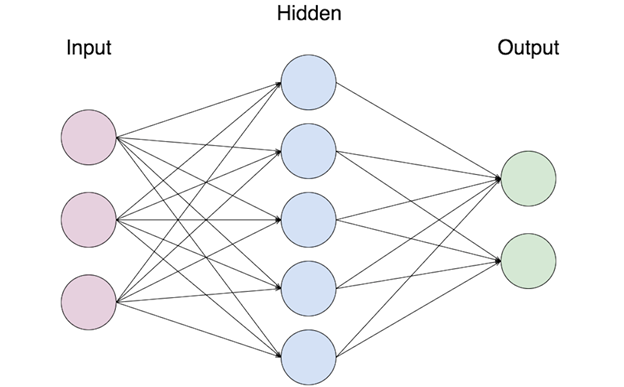
\includegraphics[scale=0.6]{img/simple-neural-network.png}
%     \caption{Mô hình mạng neural đơn giản. \cite{simple-neural-network}}
%     \label{fig:simplenn}
% \end{figure}

% Một mạng nơ-ron trước khi được đưa vào sử dụng phải trải qua quá trình huấn luyện (train) và kiểm thử (test). 
% Để thực hiện điều này, cần phải cung cấp các giá trị đầu vào và đầu ra chuẩn tương ứng. 
% Sau mỗi vòng lặp trong quá trình huấn luyện, mạng nơ-ron được kỳ vọng sẽ cho ra kết quả dự đoán gần với kết quả thực tế, 
% nói cách khác, sai số giữa đầu ra dự đoán và đầu ra chuẩn là nhỏ. Để đo lường sai số này, người ta sử dụng một hàm 
% số gọi là hàm mất mát (loss function), giá trị của hàm này được gọi là giá trị mất mát (loss). 
% Quá trình huấn luyện sẽ giảm giá trị mất mát bằng cách áp dụng giải thuật lan truyền ngược (Backpropagation) 
% kết hợp với các giải thuật tối ưu hóa như Gradient Descent, các giải thuật này sẽ được giải thích kỹ hơn ở các phần sau.

% \subsubsection*{Deep neural network }
% Mạng nơ-ron sâu (deep neural network) là một dạng mạng nơ-ron chứa nhiều lớp ẩn (hidden layer). 
% Mạng nơ-ron sâu có thể học được các bài toán phức tạp hơn so với mạng nơ-ron nông.

% \subsubsection*{ Hàm mất mát }
% Để đo lường sai số giữa đầu dự đoán của mạng nơ-ron so với đầu ra chuẩn, người ta sử dụng một hàm số gọi là hàm mất mát.
%  Giá trị của hàm số này càng nhỏ, thì mạng nơ-ron dự đoán càng gần với đầu ra chuẩn. Cho nên, nhìn chung, 
%  mục tiêu của quá trình huấn luyện là để tối thiểu hóa giá trị này. Giải thuật thường được áp dụng để giúp đạt 
%  được mục tiêu này là Gradient Descent.

% \subsubsection*{ Gradient Descent }
% Là một giải thuật nhằm tìm kiếm điểm cực tiểu của hàm số. Giải thuật này thường được sử dụng trong lĩnh 
% vực học máy nhằm giúp tối ưu hóa hàm mất mát. Giải thuật này được thực hiện bằng cách tính đạo hàm riêng 
% của giá trị mất mát so với từng tham số của mô hình, sau đó điều chỉnh các tham số này theo giá trị đạo hàm tính được. 
% Công thức để điều chỉnh như sau:

% \[ w = w - \alpha * \Delta w\]
% Trong đó: \\
% $ w $: tham số của mô hình \\
% $ \alpha $: hệ số học (learning rate) \\
% $ \Delta w $: đạo hàm của hàm mất mát theo w \\

% Để minh họa cho công thức trên, ta xem một ví dụ cho đồ thị hàm mất mát $J(w)$ với $w$ là một tham số của mạng nơ-ron (hình ~\ref{fig:gradient} . \cite{gradient-descent}

% Ta biết rằng, tại điểm cực tiểu của hàm $J$, giá trị đạo hàm bằng 0, với các điểm bên trái điểm cực tiểu, giá trị đạo hàm < 0, với các điểm bên phải, giá trị đạo hàm > 0. Như vậy, với các điểm $w$ nằm bên trái điểm cực tiểu, ta cần tăng $w$ lên, và vì $\Delta w$ lúc này < 0, nên công thức trên đã giúp tăng giá trị $w$ lên đúng như mong đợi. Tương tự với các điểm bên phải, công thức trên cũng giúp giảm $w$ về sát với điểm cực tiểu.

% Một lưu ý là với hệ số học lớn, các bước cập nhật lớn hơn giúp mạng có thể học nhanh hơn, tuy nhiên cũng tạo ra nguy cơ là sau khi cập nhật, giá trị hàm mất mát sẽ vượt qua khỏi điểm cực tiểu, và dao động qua lại 2 bên điểm cực tiểu nhưng không thể tới được đó. Ngược lại, với hệ số học nhỏ,  mạng nơ-ron sẽ học châm hơn, nhưng có thể tiến sát tới điểm cực tiểu.

% \begin{figure}
%     \centering
%     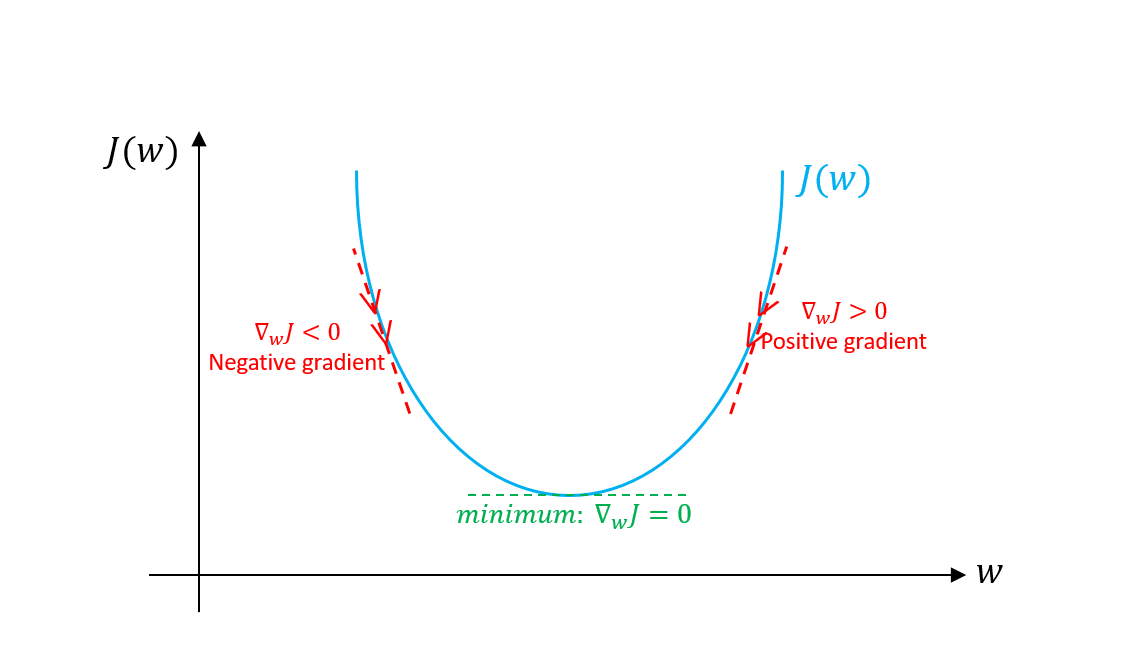
\includegraphics[scale=0.3]{img/gradient-descent.png}
%     \caption{Minh họa đồ thị hàm mất mát với Gradient descent. \cite{gradient-descent}}
%     \label{fig:gradient}
% \end{figure}
 
% \subsubsection*{ Giải thuật lan truyền ngược (Backpropogation) }

% Giải thuật chính để thực thi gradient descent trong mạng nơ-ron. Giải thuật này bao gồm 2 phần, forward pass 
% và backward pass. Ở forward pass, các giá trị đầu vào sẽ được truyền qua từng lớp nơ-ron để tính toán đầu 
% ra tương ứng. Ở mỗi lớp, các giá trị này sẽ được lưu lại để phục vụ cho việc tính toán ở backward pass. 
% Ở backward pass, mục tiêu là tính đạo hàm riêng của hàm mất mát theo từng tham số trong mỗi lớp nơ-ron. 
% Tuy nhiên, việc tính toán này không thể thực hiện một các trực tiếp, bởi vì các tham số này không xuất hiện 
% trực tiếp trong công thức tính hàm mất mát.

% Để minh họa cho giải thuật này, ta sẽ xem xét một ví dụ với một mạng nơ-ron đơn giản chỉ gồm một lớp đầu vào, 
% một lớp đầu ra cũng một lớp ẩn, mỗi lớp chỉ gồm một nơ-ron. Ở ví dụ này, ta sẽ sử dụng hàm kích hoạt là 
% sigmoid ($\sigma$), và hàm mất mát ($J$) là mean square error. Quá trình tính toán ở forward pass diễn ra như biểu diễn ở hình ~\ref{fig:forward}:

% \begin{figure}[h]
%     \centering
%     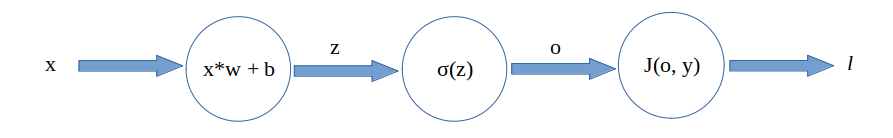
\includegraphics[scale=0.4]{img/back-propagation.png}
%     \caption{Forward pass.}
%     \label{fig:forward}
% \end{figure}

% Trong đó:\\
% $x$: giá trị đầu vào \\
% $z$: giá trị sau bước nhân tuyến tính, $ z = x * w + b $ \\
% $o$: giá trị đầu ra của nơ-ron: $ o = \sigma(z) = \frac{1}{1+e^{-z}} $ \\
% $y$: giá trị đầu ra chuẩn \\
% $l$: giá trị mất mát, $l = J(o, y) = \frac{1}{2} * (y - o)^{2}$ \\
% Viết ngắn gọn, ta có giá trị mất mát: $l = J(\sigma(x*w + b), y)$ \\
% Để có thể tính được đạo hàm của hàm $J$ theo các tham số $w$ và $b$ ta cần áp dụng Chain Rule như sau:
% \[ \Delta w = \frac{\partial l}{\partial w} = \frac{\partial l}{\partial o} * \frac{\partial o}{\partial z} * \frac{\partial z}{\partial w} \]
% \[ \Delta b = \frac{\partial l}{\partial b} = \frac{\partial l}{\partial o} * \frac{\partial o}{\partial z} * \frac{\partial z}{\partial b} \]
% Thực hiện các bước biến đổi cho công thức tính $\Delta w$ ở trên:
% \begin{equation*} \label{eq1}
% \begin{split}
% \Delta w & = \frac{\partial l}{\partial o} * \frac{\partial o}{\partial z} * \frac{\partial z}{\partial w} \\
%     & = (o - y) * (o * (1 - o)) * x  \\
% \end{split}
% \end{equation*}

% Tương tự, với tham số b của nơ-ron, ta cũng tính được $\Delta b$:
% \begin{equation*} \label{eq2}
% \begin{split}
% \Delta b & = \frac{\partial l}{\partial o} * \frac{\partial o}{\partial z} * \frac{\partial z}{\partial b} \\
%     & = (o - y) * (o * (1 - o)) \\
% \end{split}
% \end{equation*}

% Đối với ví dụ trên, nếu gọi $\Delta o$ là đạo hàm riêng của hàm mất mát theo o, $\phi(x*w + b)$ là hàm kích hoạt của nơ-ron, ta sẽ có 
% công thức tổng quát cho việc tính  $\Delta w$,  $\Delta b$ là:
% \[ \Delta w =  \Delta o * \phi ’(x*w + b) * x \]
% \[ \Delta b =  \Delta o * \phi ’(x*w + b) \]

% Với mạng nơ-ron có nhiều lớp hơn, ta cũng thực hiện tương tự các phép biến đổi này sẽ giúp tính được 
% đạo hàm của hàm mất mát theo các tham số trong từng lớp nơ-ron. Ngoài ra, nếu gọi $x_i$, $o_i$ tương 
% ứng là đầu vào và đầu ra của lớp nơ-ron thứ $i$, ta dễ dàng nhận thấy $\Delta o_i = \Delta x_i+1$, 
% điều này giúp chúng ta tiết kiệm quá trình tính toán bằng cách lan truyền ngược giá trị $\Delta x$ 
% từ lớp sau về lớp trước. Giá trị $\Delta x$ này cũng có thể được tính bằng phương pháp tương tự như 
% trình bày ở trên.

% Qua các phần trình bày ở trên, ta có thể hiểu được cơ chế giúp cho mạng nơ-ron sâu có thể học được 
% bài toán phân loại với dữ liệu đầu vào và đầu ra chuẩn. Ngoài ra, còn nhiều biến thể khác cho mạng 
% học sâu và các giải thuật liên quan, tuy nhiên trong phạm vi đề tài, nhóm sẽ không đề cập tới.

% \subsubsection*{ Mạng nơ-ron tích chập }
% Là một dạng mạng nơ-ron truyền thẳng, trong đó có ít nhất một lớp tích chập. Mạng nơ-ron tích chập đã 
% đạt được các kết quả rất tốt trong một số lĩnh vực cụ thể như nhận diện hình ảnh. Mạng này cũng được 
% dùng như là một bộ trích xuất đặc trưng hình ảnh và thu về những kết quả khả quan. Mạng nơ-ron tích chập 
% hiệu quả hơn mạng nơ-ron thông thường vì mang sử dụng phép tích chập lên các hình ảnh đầu vào, qua đó giảm 
% chi phí tính toán của mạng.
% \par
% Kiến trúc của một mạng nơ-ron tích chập thường bao gồm các lớp tích chập, theo sau là các lớp pooling,
%  cuối cùng sẽ là các lớp fully-connected dùng để kết hợp các giá trị từ những lớp trước lại để cho ra 
% kết quả dự đoán.

% \begin{figure}  
%     \centering
%     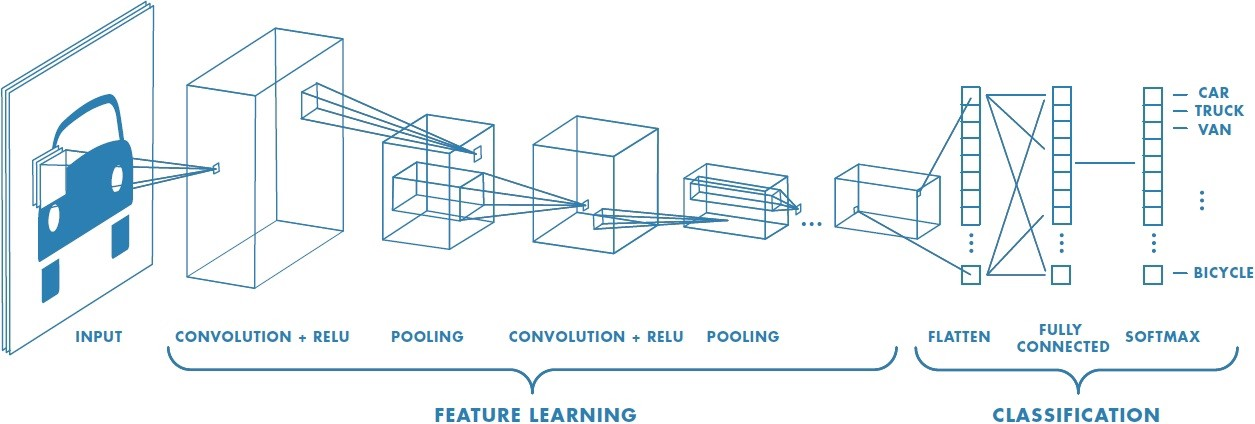
\includegraphics[scale=0.3]{img/cnn-architect.jpeg}
%     \caption{Ví dụ kiến trúc mạng nơ-ron tích chập.}
% \end{figure}    


% \subsubsection*{Lớp tích chập}
% Thay vì sử dụng phép nhân ma trận giữa các giá trị đầu vào và ma trận trọng số như mạng nơ-ron thông thường, 
% lớp tích chập sử dụng phép tính chập để tính giá trị đầu ra. Các ma trận trọng số, hay còn gọi là filter 
% này sẽ được sử dụng để quét qua từng phần của hình ảnh đầu vào để tạo ra các giá trị trong ma trận đầu ra.  
% Mỗi ô của ma trận đầu ra được tính theo công thức như sau:

% \[ Y(u,v) = X*W = \sum_{i=-r}^{r} \sum_{j=-r}^{r} X(u - i,v - j)W(i,j) \]
% Trong đó: \\
% Y: Ma trận đầu ra \\
% X: Ma trận đầu vào (hình ảnh) \\
% W: Ma trận filter được sử dụng cho phép tích chập

% Ngoài ra, filter có thể được quét qua ảnh theo bước trượt (stride) khác nhau,và ảnh đầu vào cũng có thể được thêm các giá trị đệm ở viền (padding), thường là 0 nhằm điều chỉnh kích thước ma trận. Dựa vào các thông số đầu vào, ta có thể tính kích thước ma trận đầu ra tương ứng như sau:

% \[ W_o = (W_i - F + 2P) / S + 1 \]
% \[ H_o = (H_i - F + 2P) / S + 1 \]
% \[ D_o = K \]
% Trong đó: \\
% $ W_i, H_i $: chiều rộng, chiều cao của ma trận đầu vào \\
% $ W_o, H_o, D_o $: chiều rộng, chiều cao, chiều sâu của ma trận đầu ra \\
% $ F $: kích thước một cạnh của filter \\
% $ S $: bước trượt \\
% $ P $: padding \\
% $ K $: số lượng filter \\

% Sau khi được tính bằng phép tích chập, ma trận đầu ra sẽ được đi qua hàm kích hoạt ReLu nhằm tạo 
% tính phi tuyến cho mạng nơ-ron. Công thức của hàm ReLU như sau:
% \[ y = max(x, 0). \]
% So với các hàm kích hoạt thường dùng khác như sigmoid hay tanh, hàm ReLU cho khả năng tính toán nhanh hơn, 
% cùng với đó là giải quyết vấn đề triệt tiêu đạo hàm khi x > 0.

% \subsubsection*{Lớp pooling}

% Thay vì sử dụng phép nhân ma trận giữa các giá trị đầu vào và ma trận trọng số như mạng nơ-ron thông thường, 
% lớp tích chập sử dụng phép tính chập để tính giá trị đầu ra. Các ma trận trọng số, hay còn gọi là filter 
% này sẽ được sử dụng để quét qua từng phần của hình ảnh đầu vào để tạo ra các giá trị trong ma trận đầu ra.  
% Mỗi ô của ma trận đầu ra được tính theo công thức như sau:

% \[ Y(u,v) = X*W = \sum_{i=-r}^{r} \sum_{j=-r}^{r} X(u - i,v - j)W(i,j) \]
% Trong đó: \\
% Y: Ma trận đầu ra \\
% X: Ma trận đầu vào (hình ảnh) \\
% W: Ma trận filter được sử dụng cho phép tích chập

% Ngoài ra, filter có thể được quét qua ảnh theo bước trượt (stride) khác nhau, và ảnh đầu vào cũng có 
% thể được thêm các giá trị đệm ở viền (padding), thường là 0 nhằm điều chỉnh kích thước ma trận. Dựa vào 
% các thông số đầu vào, ta có thể tính kích thước ma trận đầu ra tương ứng như sau:

% \[ W_o = (W_i - F + 2P) / S + 1 \]
% \[ H_o = (H_i - F + 2P) / S + 1 \]
% \[ D_o = K \]

% Trong đó: \\
% $ W_i, H_i $: chiều rộng, chiều cao của ma trận đầu vào \\
% $ W_o, H_o, D_o $: chiều rộng, chiều cao, chiều sâu của ma trận đầu ra \\
% $ F $: kích thước một cạnh của filter \\
% $ S $: bước trượt \\
% $ P $: padding \\
% $ K $: số lượng filter \\

% Sau khi được tính bằng phép tích chập, ma trận đầu ra sẽ được đi qua hàm kích hoạt ReLu nhằm tạo 
% tính phi tuyến cho mạng nơ-ron. Công thức của hàm ReLU như sau:
% \[ y = max(x, 0). \]
% So với các hàm kích hoạt thường dùng khác nhưu sigmoid hay tanh, hàm ReLU cho khả năng tính toán nhanh hơn, 
% cùng với đó là giải quyết vấn đề triệt tiêu đạo hàm khi x > 0.
% \subsubsection*{Lớp fully-connected}
% Lớp này có nhiệm vụ kết hợp tất cả giá trị ở các nơ-ron ở lớp trước lại, tương tự như mạng nơ-ron thông thường. 
% Ở lớp này, phép nhân ma trận được sử dụng để tạo các giá trị đầu ra. Lớp cuối cùng của một mạng nơ-ron tích 
% chập là một lớp fully-connected có số nơ-ron bằng với số class trong bài toán phân loại, hàm kích hoạt của 
% lớp này thường là hàm softmax, đây là một hàm số giúp phân hóa giá trị đầu ra về gần 2 điểm 0 và 1 hơn.

% \subsubsection*{ Học chuyển giao }
% Học chuyển giao (transfer learning) là phương pháp sử dụng các mô hình mạng nơ-ron được huấn luyện 
% sẵn để huấn luyện lại trên một tập dữ liệu mới. Việc huấn luyện lại này có thể diễn ra trên toàn bộ mạng, 
% hoặc một vài lớp nơ-ron nhất định trong mạng. Ý tưởng của phương pháp này là sử dụng các trọng số đã được 
% huấn luyện sẵn sẽ giúp mô hình học được nhanh hơn so với việc khởi tạo các giá trị trọng số này một cách
%  ngẫu nhiên. Tuy nhiên khi thực hiện học chuyển giao trên một tập dữ liệu mới, chúng ta cũng phải lưu ý 
%  lựa chọn các lớp nơ-ron nào cần được huấn luyện lại, và chọn hệ số học của mô hình phù hợp để tránh hiện 
%  tượng overfitting.
% \par 
% Ngày này, trong các bài toán sử dụng mạng nơ-ron tích chập để trích xuất đặc trưng từ ảnh, người ta 
% thường dùng các mô hình đã được huấn luyện trên tập ImageNet để thực hiện học chuyển giao, giúp cho quá 
% trình huấn luyện diễn ra nhanh hơn và cũng hiệu quả hơn.

% \section{Các nghiên cứu liên quan}
% \subsection{Bài báo: "Deep learning for content-based image retrieval: A comprehensive study." \cite{paper-1}}

% Bài báo nghiên cứu về việc áp dụng Deep Learning cho CBIR, thông qua 2 quá trình chính: 

% \begin{itemize}
%         \item Giai đoạn 1: đào tạo một mô hình Deep Learning từ một tập lớn dữ liệu đào tạo.
%         \item Ap dụng mô hình sâu đã được training cho việc học biểu diễn đặc trưng của CBIR trong một miền mới.
% \end{itemize}

% Và kết quả thu được rất khả quan:

% \begin{itemize}
%         \item Deep CNN model được train từ trước trên tập data lớn có thể được sử dụng trực tiếp cho việc rút trích đặc trưng trong nhiệm vụ CBIR mới.
%         \item Các đặc trưng được rút ra bởi mô hình CNN được đào tạo trước có thể hoặc có thể không tốt hơn các đặc trưng thủ công truyền thống, nhưng với các lược đồ tinh chỉnh đặc trưng phù hợp, biểu diễn đặc trưng học sâu luôn vượt trội so với các đặc trưng thủ công truyền thống trên tất cả các tập dữ liệu.
%         \item Khi được áp dụng biểu diễn đặc trưng trong một domain mới, thấy rằng học tương đồng có thể tăng cường hơn nữa hiệu suất truy xuất của các đặc trưng trực tiếp của các mô hình sâu được đào tạo trước.
%         \item Cuối cùng, bằng cách đào tạo lại các mô hình sâu với phân loại hoặc mục tiêu học tương tự trên domain mới, Nhận thấy rằng hiệu suất truy xuất có thể được tăng lên đáng kể, tốt hơn nhiều so với các cải tiến do học tập tương tự "nông".

% \end{itemize}

% \subsection{Bài báo: "A simple texture feature for retrieval of medical images." \cite{paper-2}}

% Bài báo đề xuất 1 cách tiếp cận đơn giản để sử dụng các đặc trưng kết cấu của hình ảnh y tế để cho việc trích xuất. Cách tiếp cận đầu tiên tiến hành lọc những hình ảnh y tế sử dụng bộ lọc Gabor và bộ lọc Schmid và sau đó phân vùng các hình ảnh được lọc thành các bản vá không chồng lên nhau. Những hoạt động này cung cấp thông đặc trưng kết cấu của những hình ảnh y tế. Mô hình bag-of-words cuối cùng được sử dụng để có được những biểu diễn đặc trưng của những hình ảnh y tế. So với một số đặc trưng hiện có, đặc trưng được đề xuất có tính phân biệt và hiệu quả hơn. Các thí nghiệm trên hai cơ sở dữ liệu hình ảnh CT y tế đã chứng minh tính hiệu quả của phương pháp được đề xuất.

% \subsection{Bài báo: "A new method of content based medical image retrieval and its applications to CT imaging sign retrieval" \cite{paper-3}}

% Bài viết này đề xuất một phương pháp mới để thu thập hình ảnh y tế dựa trên nội dung thông qua việc xem sự tương đồng nhạy cảm ngữ cảnh, đồng nhất. Thứ nhất, nhóm nghiên cứu kết hợp các điểm tương đồng ngữ nghĩa và hình ảnh giữa hình ảnh truy vấn và từng hình ảnh trong cơ sở dữ liệu dưới dạng các điểm giống nhau của chúng. Sau đó, xây dựng một biểu đồ có trọng số có các nút đại diện cho các hình ảnh và các cạnh đo các điểm giống nhau của chúng. Bằng cách sử dụng thuật toán đường đi ngắn nhất trên biểu đồ trọng số, nhóm nghiên cứu có được một thước đo tương tự mới, đo lường tương tự về ngữ cảnh, giữa hình ảnh truy vấn và từng hình ảnh cơ sở dữ liệu để hoàn tất quá trình truy xuất. Trên thực tế, nhóm nghiên cứu sử dụng tính tương tự của cặp tương tự để thu hẹp khoảng cách ngữ nghĩa để có được một phép đo tương tự cặp đôi chính xác hơn và trải rộng trên phạm vi dữ liệu nội tại để đạt được sự giống nhau về ngữ cảnh cho hiệu suất truy xuất tốt hơn. Phương pháp đề xuất đã được đánh giá dựa trên việc rút trích các dấu hiệu hình ảnh CT phổ biến của bệnh phổi (CISLs) và đạt được không chỉ kết quả thu hồi tốt hơn mà còn đạt hiệu quả tính toán thỏa đáng.

% % Bài báo đề xuất phương pháp CBMIR mới bằng cách chụp hình học của các bản sao bên dưới. Phương pháp được đề xuất được gọi là FCSS (tương đồng nhạy cảm ngữ cảnh hợp nhất) trong thời gian ngắn. Thứ nhất, chúng ta có được sự giống nhau về ngữ nghĩa giữa hình ảnh truy vấn và hình ảnh cơ sở dữ liệu theo thông tin phân loại, sau đó tính toán các điểm tương đồng trực quan của chúng theo khoảng cách của chúng trong không gian đặc trưng trực quan. Dựa trên hai loại tương đồng ở trên, chúng ta đạt được sự tương đồng về mặt cặp đôi hợp nhất. Thứ hai, một đồ thị có trọng số liên quan đến hình ảnh truy vấn và tất cả các hình ảnh cơ sở dữ liệu được xây dựng, và đường đi ngắn nhất trên biểu đồ được tính là sự tương tự về ngữ cảnh giữa hình ảnh truy vấn và từng hình ảnh cơ sở dữ liệu. Cuối cùng, các hình ảnh cơ sở dữ liệu được xếp hạng và trả về theo sự tương đồng về ngữ cảnh nhạy cảm được hợp nhất. Chúng tôi áp dụng phương pháp CBMIR được đề xuất để lấy các dấu hiệu hình ảnh CT phổ biến của bệnh phổi (CISLs), thường xuất hiện trong các phát hiện CT phổi của bệnh nhân và đóng vai trò quan trọng trong chẩn đoán bệnh phổi.

% \subsection{Bài báo: "Deep convolutional learning for Content Based Image Retrieval" \cite{paper-4}}

% Bài báo đề xuất một phương pháp huấn luyện lại mô hình để tìm hiểu các biểu diễn convolutional hiệu quả hơn cho việc truy xuất hình ảnh dựa trên nội dung. Sử dụng mô hình Deep CNN đã được huấn luyện trước để thu được các biểu diễn tính năng từ việc kích hoạt các lớp convolutional bằng cách sử dụng max-pooling, và sau đó điều chỉnh và huấn luyện lại mạng, để tạo ra các mô tả hình ảnh nhỏ gọn hiệu quả hơn, cải thiện hiệu suất truy xuất và yêu cầu bộ nhớ, dựa vào thông tin có sẵn. 

% Các tác giả gợi ý ba phương pháp huấn luyện mô hình cơ bản. 
% Đó là:
% \begin{itemize}
%         \item Huấn luyện lại hoàn toàn không được giám sát khi không có thông tin ngoại trừ từ tập dữ liệu có sẵn. 
%         \item Huấn luyện lại với thông tin liên quan khi các nhãn của tập dữ liệu huấn luyện có sẵn.
%         \item Huấn luyện lại dựa trên phản hồi có liên quan nếu có phản hồi từ người sử dụng. 
% \end{itemize}

% Việc đánh giá thực nghiệm trên ba tập dữ liệu truy xuất hình ảnh công khai cho thấy hiệu quả của phương pháp được đề xuất trong việc học các biểu diễn hiệu quả hơn cho việc trích xuất, vượt trội hơn các kỹ thuật trích xuất dựa trên CNN khác, cũng như các phương pháp dựa trên đặc điểm thủ công truyền thống trong tất cả bộ dữ liệu đã sử dụng.




% %%%%%%%%Chapter 3 Giải thuật và đề xuát nghiên cứu%%%%%%%%%%%%%
% \chapter{Phương pháp đề xuất}
% \section{Yêu cầu bài toán}
% Yêu cầu của bài toán là hiện thực một phương pháp giúp tìm kiếm đối tượng trong một tập dữ liệu ảnh cho trước. 
% Để có thể tìm kiếm đối tượng theo đặc trưng, bài toán cũng tạo ra một yêu cầu phụ là phải tạo ra cơ sở 
% dữ liệu đặc trưng tương ứng với từng ảnh trong cơ sở dữ liệu hình ảnh, thông qua đó mới có thể so sánh 
% với hình ảnh đầu vào.

% \section{ Phương pháp đề xuất }

% \subsection{Sử dụng đặc trưng được trích xuất từ mạng nơ-ron tích chập đã được huấn luyện}
% Trong phần này, nhóm sẽ đánh giá kết quả thu được từ việc trích xuất dựa trên một mạng nơ-ron tích 
% chập đã được huấn luyện để phân loại 1000 loại hình ảnh cho tập ImageNet. Đây là phương pháp đơn 
% giản nhất khi sử dụng mạng nơ-ron tích chập để làm bộ trích xuất đặc trưng, và cũng được đã nhiều bài báo sử dụng.

% Phương pháp này dựa trên ý tưởng mạng nơ-ron sau khi được huấn luyện để có thể phân loại ảnh thì cũng sẽ cho 
% ra các đặc trưng tương tự với các bức ảnh tương tự nhau.

% Input của giải thuật này là ảnh một vật thể đã được điều chỉnh kích thước phù hợp với kích thước đầu vào của mạng nơ-ron tích chập được huấn luyện.

% Output của giải thuật là tập các ảnh trong cơ sở dữ liệu có độ tương đồng cao nhất với ảnh đầu vào.

% Sơ đồ xử lý của giải thuật được mô tả như hình 3.1, trong đó, ảnh đầu vào sẽ trải qua bước tiền xử lý đề thu về ảnh có kích thước phù hợp với đầu vào của mạng nơ-ron tích chập. Ảnh sau đó sẽ được truyền qua mạng nơ-ron để thu về vector đặc trưng, cũng chính là giá trị tại lớp fully-connected gần cuối cùng của mạng. Vector đặc trưng này sẽ được so sánh với các vector đặc trưng của ảnh trong cơ sơ dữ liệu. Dựa vào kết quả so sánh được, tập ảnh có độ tương đồng cao nhất với ảnh đầu vào sẽ được trích xuất ra.

% \begin{figure}  
%     \centering
%     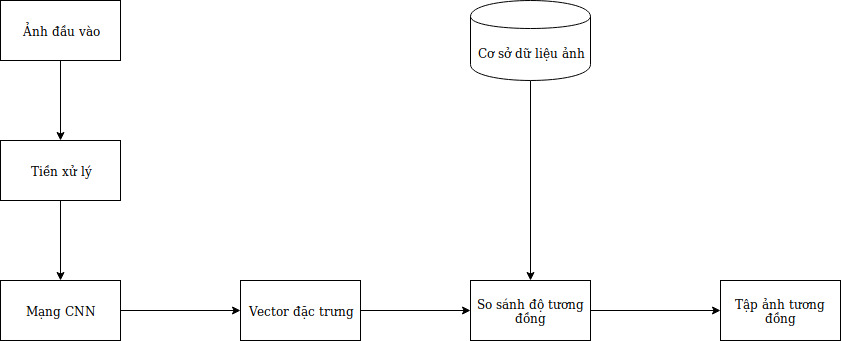
\includegraphics[scale=0.5]{img/cnn-feature-extractor.jpg}
%     \caption{Sơ đồ xử lý của giải thuật sử dụng mạng nơ-ron tích chập.}
% \end{figure}    

% Ưu điểm của phương pháp này là cho kết quả nhanh chóng, đồng thời có thể áp dụng trực tiếp lên một tập 
% dữ liệu mới mà không cần phải huấn luyện lại. Tuy nhiên có thể dễ thấy rằng việc áp dụng một mạng nơ-ron 
% được huấn luyện sẵn vào một tập dữ liệu khác với tập dữ liệu huấn luyện có thể sẽ mang đến kết quả không thực sự tốt.



% \subsection{Sử dụng đặc trưng được trích xuất từ mạng nơ-ron tích chập sau khi thực hiện học chuyển giao }

% Với phương pháp này, nhóm kỳ vọng rằng việc thực hiện học chuyển giao cho một mô hình mạng nơ-ron 
% được huấn luyện sẵn trên tập dữ liệu mới sẽ giúp mô hình đưa ra những đặc trưng gần hơn với dữ liệu, 
% thông qua đó cải thiện độ chính xác của mô hình.

% Phương pháp này tương tự như phương pháp đề xuất ở mục 3.2.1, điểm khác biệt chính là trước khi sử dụng mạng nơ-ron tích chập làm bộ trích xuất đặc trưng, nhóm sẽ thực hiện học chuyển giao trên tập dữ liệu mới. Sau đó, các đặc trưng ảnh sẽ được trích xuất tương tự như quy trình đã nêu ở mục 3.1.1.

% \section{ Các phương pháp đánh giá }
% Nhóm sẽ thực hiện đánh giá bằng cách đo lường độ chính xác của các hình ảnh được tìm thấy dựa theo nhãn 
% của hình ảnh.

% \[ \text{độ chính xác} = \frac{\text{số lượng hình ảnh tìm được với nhãn đúng}}{\text{tổng số lượng hình ảnh tìm được}} \]
% % %%%%%%%%%%%Chapter 4 Hiện thực mô hình đơn giản%%%%%%%%%%%%%%%%%%%%%    
% \chapter{Hiện thực và đánh giá kết quả}
% \section{Tài nguyên cần thiết}
% \subsection{Ngôn ngữ Python}
% % Python là ngôn ngữ lập trình thông dịch, hướng đối tượng, và là ngôn ngữ lập trình cấp cao được tạo ra bởi Guido van Rossum tại Centrum Wiskunde & Informatica (CWI) ở Hà Lan. Python là một ngôn ngữ có cú pháp đơn giản, dễ đọc hiểu, cách viết linh động, được biết như là một trong những ngôn ngữ lập trình nhập môn tốt nhất cho người bắt đầu lập trình và hiện nay đang được sử dụng rộng rãi trong nhiều lĩnh vực với nhiều mục đích khác nhau.
% % Đặc điểm của ngôn ngữ Python
% \begin{itemize}
%         \item Ngôn ngữ lập trình đơn giản, dễ học: Python có cú pháp rất đơn giản, rõ ràng. Nó dễ đọc và viết hơn rất nhiều khi so sánh với những ngôn ngữ lập trình khác như C++, Java, C#. Python làm cho việc lập trình trở nên thú vị, cho phép bạn tập trung vào những giải pháp chứ không phải cú pháp.
%         \item Miễn phí, mã nguồn mở: Ta có thể tự do sử dụng và phân phối Python, Python có một cộng đồng rộng lớn và không ngừng cải thiện.
%         \item Là ngôn ngữ dynamic type, quản lý vùng nhớ tự động và hỗ trợ nhiều mô hình lập trình khác nhau như: lập trình hướng đối tượng, lập trình thủ tục và lập trình hàm. Là một ngôn ngữ rất phổ biến và có một lượng lớn các thư viện hỗ trợ như OpenCV, Numpy, Scikit, TensorFlow,...
%         \item Python là ngôn ngữ có thể chạy trên nhiều nền tảng: Python có trên mọi hệ điều hành như Windows, Linux/Unix, OS/2, Mac, Amiga, và những hệ điều hành khác.
% \end{itemize}

% Ngoài những ưu điểm trên, lý do quan trọng nhất để nhóm chọn ngôn ngữ Python là vi ngôn ngữ Python có framework Tensorflow, một framework vô cùng mạnh mẽ và tiện lợi cho việc hiện thực và đánh mô hình mà nhóm đã lựa chọn.

% \subsection{Framework TensorFlow}



% \section{Hiện thực các module}
% Trong quá trình thử nghiện, nhóm sử dụng kết một phần nhỏ của bộ dữ liệu CALTECH101 và Standford Cars Dataset để tạo ra một bộ dữ liệu gồm 4 loại phương tiện di chuyển: Airplane, Car, Ketch, Motobike. Vì mục đích tạo ra kết quả nhanh và giới hạn độ phức tạp của dữ liệu, nhóm đã chọn ra mỗi loại phương tiện 110 hình mẫu, chia thành 2 tập huấn luyện gồm 90 hình/nhãn, và kiểm thử gồm 20 hình/nhãn.

% Dưới đây là một số hình mẫu trong tập dữ liệu huấn luyện của nhóm.
% \begin{figure}
%     \centering
%     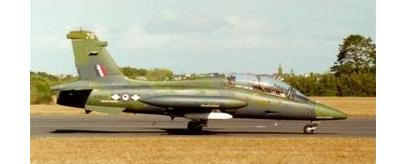
\includegraphics[scale=1]{img/airplane-sample.jpg}
%     \caption{Hình mẫu một chiếc máy bay phản lực.}
%     \label{fig:arplane-sample}
% \end{figure}
% \begin{figure}
%     \centering
%     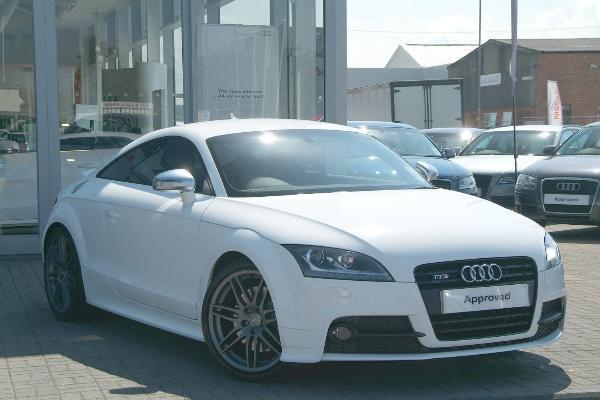
\includegraphics[scale=0.5]{img/car-sample.jpg}
%     \caption{Hình mẫu một chiếc xe hơi.}
%     \label{fig:car-sample}
% \end{figure}
% \begin{figure}
%     \centering
%     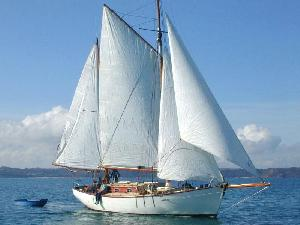
\includegraphics[scale=1]{img/ketch-sample.jpg}
%     \caption{Hình mẫu một chiếc thuyền buồn.}
%     \label{fig:ketch-sample}
% \end{figure}

% \begin{figure}
%     \centering
%     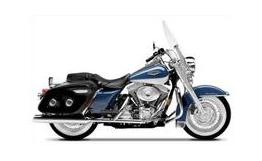
\includegraphics[scale=1]{img/motobike-sample.jpg}
%     \caption{Hình mẫu một chiếcxe moto.}
%     \label{fig:moto-sample}
% \end{figure}







% \section{Quy trình thực hiện}
% Nhóm sử dụng mạng Alexnet đã được huấn luyện trên bộ ImageNet để thử nghiệm bằng hai phương pháp:
% \par
% Sử dụng trực tiếp Alexnet làm bộ trích xuất đặc trưng cho hình ảnh.
% \par
% Thực hiện tinh chỉnh và học chuyển giao trên Alexnet trước khi sử dụng làm bộ trích xuất đặc trưng.
% \par
% Ở cả hai phương pháp, nhóm đều sử dụng output ở lớp fully-connected gần cuối (lớp FC7 trong mô hình mạng Alexnet) làm vector đặc trưng và đo lường độ tương đồng bằng khoảng cách Euclid.
% \par
% Để đánh giá kết quả hiện thực, nhóm sẽ tính độ chính xác dựa theo độ chính xác khi so sánh với nhãn của dữ liệu.
% \section{Kết quả}

% Kết quả thực nghiệm trên tập dữ liệu của nhóm cho độ chính xác 91\% đối với phương pháp thực hiện học chuyển giao và 92\% đối với phương pháp sử dụng trực tiếp alexnet. 
% Nhìn chung kết quả này chưa thể khẳng định được phương pháp nào tốt hơn, vì tập dữ liệu 
% tương đối nhỏ và chưa được làm giàu để tránh overfitting. Tuy vậy những kết quả này cũng 
% giúp nhóm hiểu hơn về cách mà mạng nơ-ron tích chập được sử dụng để trích xuất đặc trưng 
% của ảnh.

% Hình 4.5, 4.6, 4.7 cho thấy kết quả thử nghiệm của nhóm với 2 phương pháp đề xuất ở chương 3. Các kết quả tìm được của 2 phương pháp có sự trùng lặp với nhau.

% \begin{figure}
%     \centering
%     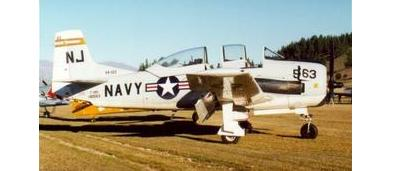
\includegraphics[scale=1]{img/ariplane-query.jpg}
%     \caption{Ảnh đầu vào}
% \end{figure}

% \begin{figure}
%     \centering
%     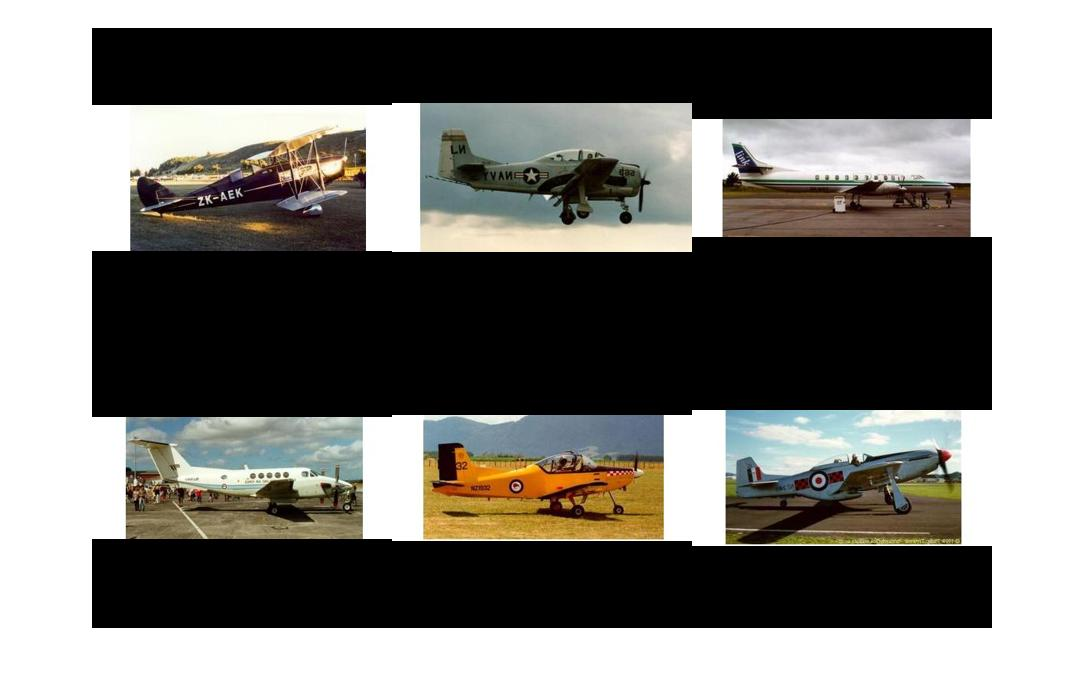
\includegraphics[scale=0.4]{img/airplane_query_by_similarity_no_transfer.jpg}
%     \caption{Top 6 ảnh tìm được không sử dụng học chuyển giao}
% \end{figure}

% \begin{figure}
%     \centering
%     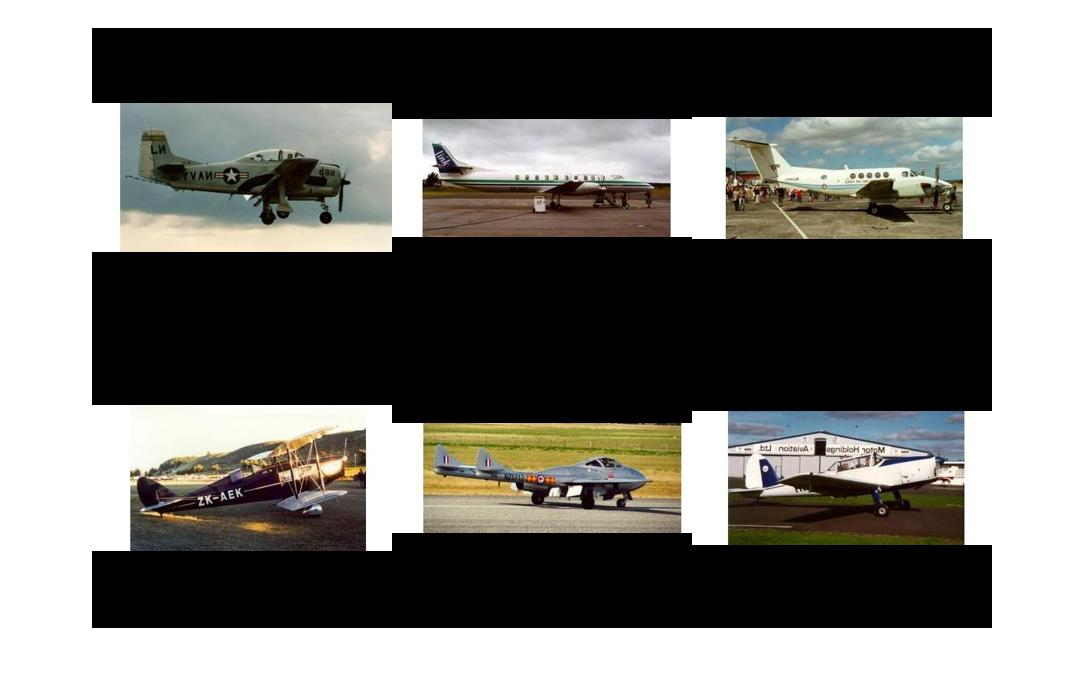
\includegraphics[scale=0.4]{img/airplane_query_by_similarity.jpg}
%     \caption{Top 6 ảnh tìm được có sử dụng học chuyển giao}
% \end{figure}



% %%%%%%%%%%%Chapter 5 Kết luận%%%%%%%%%%%%%%%%%%%%%
% \chapter{Kết luận}
% \section{Kết quả đạt được}

% Với các nội dung trình bày ở các phần trên, nhóm đã hoàn thành được các mục tiêu trong giai đoạn đề cương luận văn này:
% \begin{itemize}
%     \item Tìm hiểu được cơ sở lý thuyết về hình ảnh số.
%     \item Tìm hiểu các đặc trưng của hỉnh ảnh số cũng như các giải thuật trích xuất đặc trưng này.
%     \item Tìm hiểu được cơ sở lý thuyết cho mạng nơ-ron, thông qua đó hiểu được hướng áp dụng mạng nơ-ron tích chập vào bài toán
%     \item Hiện thực được một ứng dụng đơn giản để quan sát các kết quả bước đầu
%     \item Biết được các ưu nhược điểm của phương pháp, qua đó hiểu rằng cần phải tìm hiểu thêm để tìm cách khắc phục.
% \end{itemize}

% \section{Ưu nhược điểm}

% \subsection{Ưu điểm}

% \begin{itemize}
%     \item Không sử dụng các phương pháp trích xuất đặc trưng thủ công.
%     \item Kết quả thử nghiệm tương đối cao.
% \end{itemize}

% \subsection{Nhược điểm}

% \begin{itemize}
%     \item Thời gian tính toán và không gian bộ nhớ cần để lưu trữ vector đặc trưng cao.
% \end{itemize}

% \section{Định hướng luận văn tốt nghiệp}

% Tiếp tục tìm hiểu về lĩnh vực này. Hiện thực các phương pháp đề xuất và thực hiện so sánh với các phương pháp truyền thống. Hiện thực website hoàn thiện để minh họa cho ứng dụng.

% % %%%%%%%%%%%%%%%%%%%%%%%%%%%%%%%%%
% \medskip
% \bibliographystyle{unsrt}
% \begin{thebibliography}{9}

% \bibitem{img-defi}
% Isaac Weiss. Digital Images. Truy xuất từ: \texttt{\burl{https://www.encyclopedia.com/computing/news-wires-white-papers-and-books/digital-imageas}}

% \bibitem{img-format}
% Nguyễn Kiên. Tìm hiểu về các định dạng hình ảnh. Truy xuất từ: \texttt{\burl{https://blogchiasekienthuc.com/thu-thuat-hay/tim-hieu-ve-cac-dinh-dang-hinh-anh.html}}

% \bibitem{rgb}
% Adrien Ulens. \textit{CMYK vs. RGB - what is the difference?} Truy xuất từ: \\\texttt{\burl{lhttps://www.gogoprint.sg/blog/cmyk-vs-rgb-sg/}}

% \bibitem{simple-neural-network}
% BLog Code từ đầu. \textit{Neural Network và Deep Learning là gì?} Truy xuất từ: \texttt{\burl{https://codetudau.com/neural-network-va-deep-learning-la-gi/index.html}}

% \bibitem{gradient-descent}
% Imad Dabbura. \textit{Gradient Descent Algorithm and Its Variants.} Truy xuất từ: \\\texttt{\burl{https://towardsdatascience.com/gradient-descent-algorithm-and-its-variants-10f652806a3}}

% \bibitem{application-cbir}
% OLDOC, Free On-Line Dictionary Of Computing, “co-occurrence matrix,” May 1995, Truy xuất từ: \texttt{\burl{http://foldoc.doc.ic.ac.uk/foldoc/foldoc.cgi?cooccurrence+matrix}}

% \bibitem{cbir-defi}
% Vipin Tyagi,\textit{ContentBased Image Retrieval: Ideas, Influences, and Current Trends}, trang 4, 2017.


% \bibitem{features}
% Kranthi Kumar. CBIR: Content Based Image Retrieval. \textit{National Conference on Advances in Information Security(NCAIS-2010)}

% \bibitem{class-tt}
% Vipin Tyagi, ContentBased Image Retrieval: Ideas, Influences, and Current Trends, trang 11, 2017


% \bibitem{spatial}
% Vipin Tyagi, \textit{ContentBased Image Retrieval: Ideas, Influences, and Current Trends}, trang 16, 2017
% \bibitem{level-cbir}
% Ying Liua, Dengsheng Zhanga. \textit{A survey of content-based image retrieval with high-level semantics},  April 2006

% \bibitem{paper-1} 
% Ji WAN, Dayong WANG, Steven C. H. HOI, Pengcheng WU, Jianke ZHU, Yongdong ZHANG, and Jintao LI.
% Deep learning for content-based image retrieval: A comprehensive study.
% \textit{Research Collection School Of Information Systems, Institutional Knowledge at Singapore Management University}, 2014.
 
% \bibitem{paper-2} 
% Rushi Lan, Si Zhong, Zhenbing Liu, Zhuo Shi, and Xiaonan Luo.
% A simple texture feature for retrieval of medical images.
% \textit{Multimedia Tools and Applications}, 2017.
 
% \bibitem{paper-3} 
% Ling Ma, Xiabi Liu, Yan Gao, Yanfeng Zhao, Xinming Zhao, Chunwu Zhou. A new method of content based medical image retrieval and its applications to CT imaging sign retrieval.
% \textit{Journal of Biomedical Informatics}, 2017.

% \bibitem{paper-4} 
% Maria Tzelepi and Anastasios Tefas. Deep convolutional learning for Content Based Image Retrieval.
% \textit{Neurocomputing}, 2017.
% \end{thebibliography}
\end{document}


